\documentclass[25pt, a1paper, portrait]{tikzposter}

\usepackage{graphicx}
\usepackage{wrapfig}
\usepackage{hyperref}
\usepackage{cabin}  % cabin font
\renewcommand{\familydefault}{\sfdefault}
\settitle{}

\tikzposterlatexaffectionproofoff
\AtBeginDocument{%
    \begin{pgfonlayer}{backgroundlayer}
        \node[
            inner sep=4pt, anchor=south east, fill=white, draw=none,
            rounded corners=5, fill opacity=0.3, text opacity=1
        ] at (0.5\textwidth-7pt, -0.5\textheight+7pt)
        {\small{\textrm\LaTeX}~\textrm{Ti\emph{k}Z}\textrm{poster} – \href{https://github.com/mstimberg/joss-poster}{github.com/mstimberg/joss-poster}};
    \end{pgfonlayer}
}

% https://tex.stackexchange.com/questions/254257/tikzposter-and-doi-package-conflict
\def\HyperFirstAtBeginDocument#1{#1}
\begin{document}

\makeatletter
    \setlength{\TP@blocktop}{.49\textheight}
\makeatother

\block[linewidth=0pt]{}{
	\begin{minipage}[c]{0.6\textwidth}
    \includegraphics[width=\textwidth]{joss-logo-transparent-crop.png}
  	\end{minipage}
  	\hspace{0.04\textwidth}
  	\begin{minipage}[c]{0.3\textwidth}
    \textbf{Editorial board} \\
    Arfon Smith \emph{(Editor-in-Chief)}\\
    Dan Foreman-Mackey\\
    Olivia Guest\\
    Daniel S.~Katz\\
    Kevin M.~Moerman\\
    Kyle Niemeyer\\
    Kristen Thyng\\
    \\
    {\Huge{\href{https://joss.theoj.org}{\ttfamily joss.theoj.org}}}
  	\end{minipage}
\par\vspace{1em}
Presented by \textbf{Marcel Stimberg} (JOSS Topic Editor) at the \emph{Neuroscience Open Worshop 2023} (22--23 Nov 2023)
}

\begin{columns}
\column{0.5}

\block{}{The Journal of Open Source Software (JOSS)
  is an \textbf{academic journal} (ISSN 2475-9066) that publishes short
  articles describing \textbf{open source research software}.  The review process includes checking that the
  software itself
  \href{https://joss.readthedocs.io/en/latest/review_checklist.html}{\bfseries meets
    modern standards}, including having documentation, tests
  (preferably automated), and community guidelines.  This way, JOSS
  aims to give software creators a \textbf{citable artefact}
  through which their research contribution can be recognised,
  and to encourage them to use \textbf{good software practice}.
}

\block{Publication statistics}{
  \begin{center}
    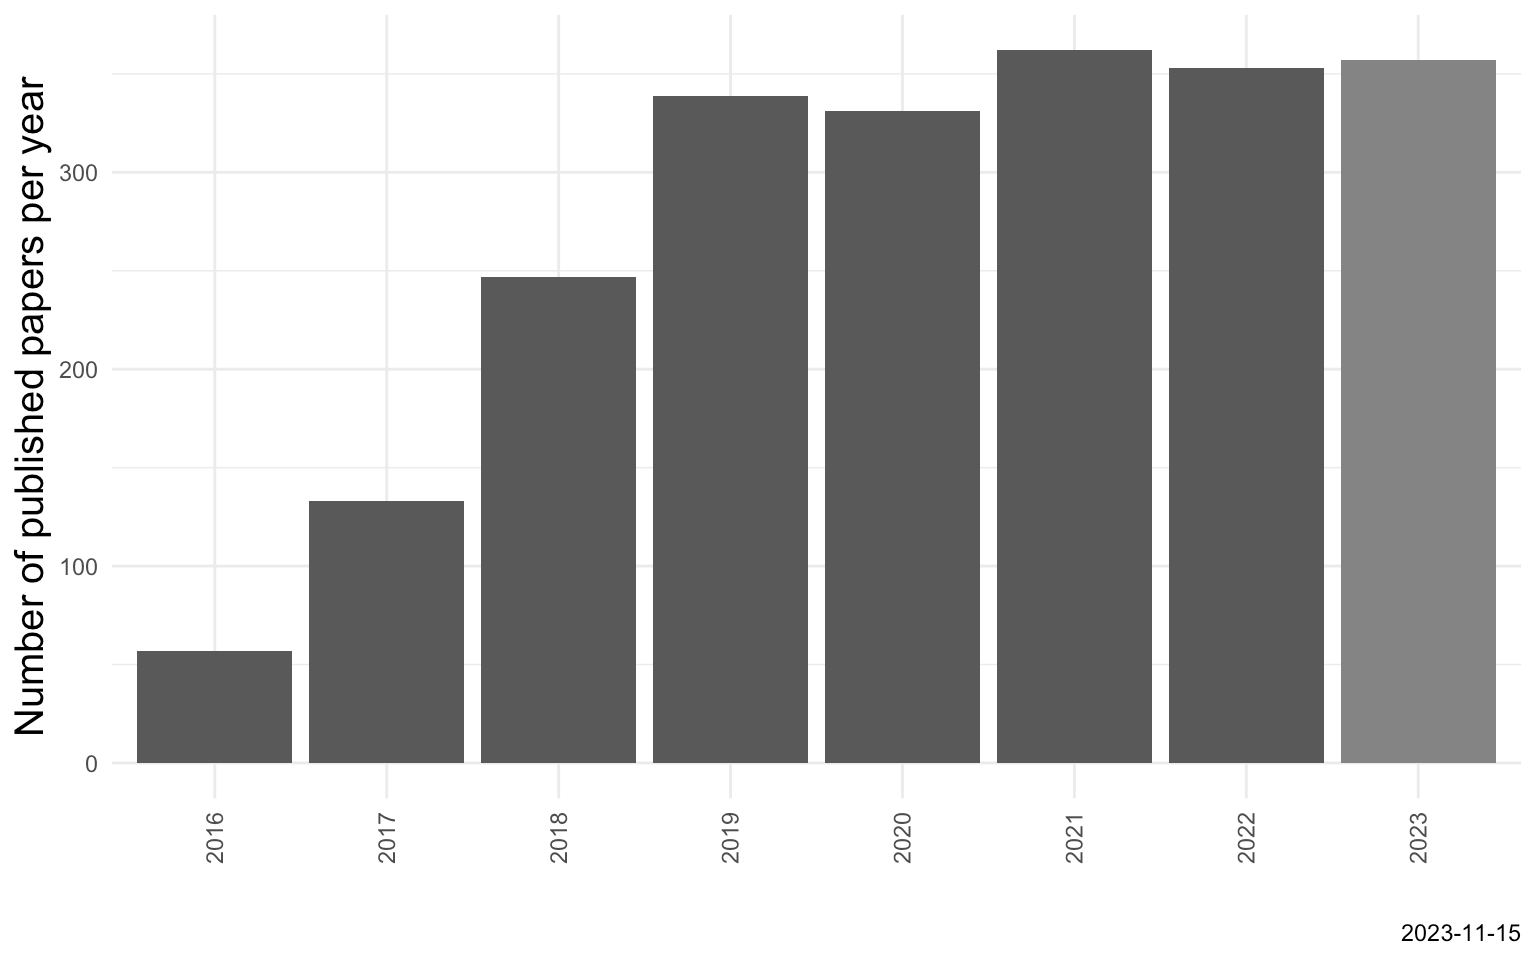
\includegraphics[width=0.4\textwidth]{joss-papers-per-year.png}
  \end{center}
  \begin{center}
    \emph{Most-cited articles}:
   \small{
  \begin{tabular}{p{0.7\linewidth}@{\quad}cr}
    \textbf{Title} & \textbf{Year} & \textbf{Citations} \\
    \href{http://dx.doi.org/10.21105/joss.01686}{Welcome to the Tidyverse} & 2019 & 6\,747 \\
    \href{http://dx.doi.org/10.21105/joss.00861}{UMAP: Uniform Manifold Approximation and Projection}
    & 2018 & 3\,618 \\
    \href{http://dx.doi.org/10.21105/joss.03021}{seaborn: statistical data visualization} & 2021 & 1\,678 \\
    \href{http://dx.doi.org/10.21105/joss.00024}{corner.py: Scatterplot matrices in Python} & 2016 & 1\,081 \\
    \href{http://dx.doi.org/10.21105/joss.03139}
         {performance: An R Package for Assessment, Comparison and Testing of Statistical Models}
         & 2021 & 915 \\
  \end{tabular}
  }
  \end{center}
}

\block{Get involved}{
  \textbf{Publish your code! \href{https://joss.readthedocs.io/en/latest/submitting.html}{\small{joss.readthedocs.io/en/latest/submitting.html}}}\\
  JOSS is developer-friendly.  If you've already developed a significant research code with an open source licence, good documentation and tests, it should not take much to prepare and submit your paper to JOSS.
  \\
  \textbf{Volunteer to review! \href{https://reviewers.joss.theoj.org/join}{\small{reviewers.joss.theoj.org/join}}}\\
  The review process is an opportunity to help creators improve their software.
  Reviewers are encouraged to open issues and iteratively improve the software, rather
than providing a few monolithic reviews, several weeks apart.}

\column{0.5}
\block{Publication workflow}{
  \begin{center}
    \includegraphics[width=0.42\textwidth]{JOSS-flowchart-updated.pdf}
  \end{center}
}

\block{Behind the scenes}
{JOSS streamlines its editorial processes by using software
  development tools.  Pre-review and review discussions happen in
  \textbf{GitHub issues}.  Many editorial steps are handled by the \textbf{editorial
  bot}: a \href{https://buffy.readthedocs.io/}{Ruby package}
  that interacts with GitHub via its API to do editorial tasks
  like recompiling the article PDF on request, checking reference DOIs, and more! \\
  \\
  Manuscripts are prepared in a flavour of \textbf{Markdown} and compiled to
  PDF via Pandoc.  JOSS's compilation process is available to authors
  as a GitHub action, so compliance can be checked automatically.
}

  \block[roundedcorners=0]{}{
  \small{
Based on a poster by Warrick Ball (\href{https://github.com/warrickball/joss-poster}{github.com/warrickball/joss-poster}).  Publication workflow diagram by Kyle Niemeyer. \\

Licensed under a CC By 4.0 License: \\
\url{http://creativecommons.org/licenses/by/4.0/}}
\begin{wrapfigure}[5]{r}{7.5cm}\vskip-4em\includegraphics[width=\linewidth]{by.png}\end{wrapfigure}
}
\end{columns}


\end{document}
